\section{Структура индексов в MySQL InnoDB}

Индексы представляют собой структуры, которые помогают эффективно извлекать данные.
В СУБД MySQL InnoDB используются Btree индексы, основанные на структуре данных B+tree Рисунок \ref{img:btree-structure}.

\begin{figure}[H]
  \centering
  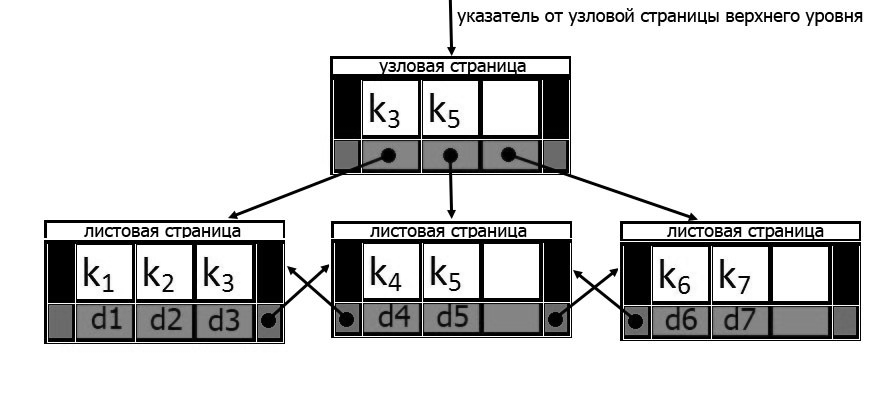
\includegraphics[scale=0.5]{btree.png}
  \caption{Структура данных B+tree.}
  \label{img:btree-structure}
\end{figure}

Где
$k_i$ - ключи ($k_i < k_i + 1$),
$d_i$ - данные.

Сложность поиска в линейной структуре данных $O(N)$, а в B+tree - $log(k)+N_k$, где $k$ — количество уровней, а $N_k$ — количество элементов в узле. Поэтому индексы, использующие структуру данных B+tree, эффективны для поиска данных. Для оптимизации поиска по диапазону в листовых страницах есть указатели на следующую и предыдущую листовую страницу.

В качестве примера рассматрим таблицу $$poet (poet\_id, last\_name, first\_name, dob, country)$$

\begin{table}[h]
\caption{Таблица поэтов}
\medskip
\begin{tabular}{|l|l|l|l|l|}
\hline
poet\_id & last\_name & first\_name & dob & country\\
\hline
1 & "Блок" & "Александр" & 1880 & "ru"\\
2 & "Фет" & "Афанасий" & 1820 & "ru"\\
3 & "Лермонтов" & "Михаил" & 1814 & "ru"\\
4 & "Ильф" & "Илья" & 1897 & "ru"\\
5 & "Пушкин" & "Александр" & 1799 & "ru"\\
6 & "Булгаков" & "Михаил" & 1891 & "ru"\\
7 & "Есенин" & "Сергей" & 1895 & "ru"\\
\hline
\end{tabular}
\end{table}

\subsection{Кластерный индекс}

В InnoDB данные хранятся в структуре B+tree, где в узловых страницах хранятся первичные ключи, а в листовых страницах хранятся данные. Такое дерево называется кластерным индексом. Над таблицей можно построить только один кластерный индекс, поскольку невозможно хранить одну и ту же запись одновременно в двух местах. Однако часть или всю запись можно хранить в нескольких местах, что будет использоваться в покрывающих индексах \ref{section:covering-index}.

По рисуноку \ref{img:btree-structure}, где $k_1 \ldots k_7$ - первичные ключи ($poet\_id$), $k_i = i$; $d_1 \ldots d_7$ - данные.

$d_1$ = Блок, Александр, 1880, ru; 

$d_2$ = Фет, Афанасий, 1820, ru;

$\ldots$

Если вы не задаёте первичный ключ, то MySQL неявно добавит скрытое поле и кластерезует данные по нему, но доступа к нему не даст. Отсюда следует, что первичный ключ желательно явно создавать самим.

Характерной проблемой кластерного индекса является то, что при вставке в страницу, если в ней закончилось место, создается новая пустая страница. Из-за этого, со временем появляется много пустующего места и таблицы InnoDB начинают занимать много места. Данная проблема решается командой $OPTIMAZE\:TABLE\;table\_name;$

\subsection{Вторичный индекс}

Для оптимизации конкретных запросов используются вторичные индексы (далее просто индексы). В узловых страницах индексов хранятся поля, по которым создан этот индекс, а в листовых страницах хранится значение первичного ключа. Для каждой таблицы в одном запросе используется только один индекс. При использовании в запросах индекса, сначала будет найдено значение первичного ключа, затем по этому значению будут найдены данные в кластерном индексе. Поэтому при создании вторичного индекса, в конец неявно добавляется первичный ключ.

На рисунке \ref{img:index-structure} показан индекс по полю (dob). Где $k_1 \ldots k_7$ - ключи, по которым построен индекс; $k_1$ = 1799, $k_2$ = 1814, $k_3$ = 1820, $\ldots$; $p_1 \ldots p_7$ - первичные ключи ($poet\_id$); $p_i = i$.

\begin{figure}[H]
  \centering
  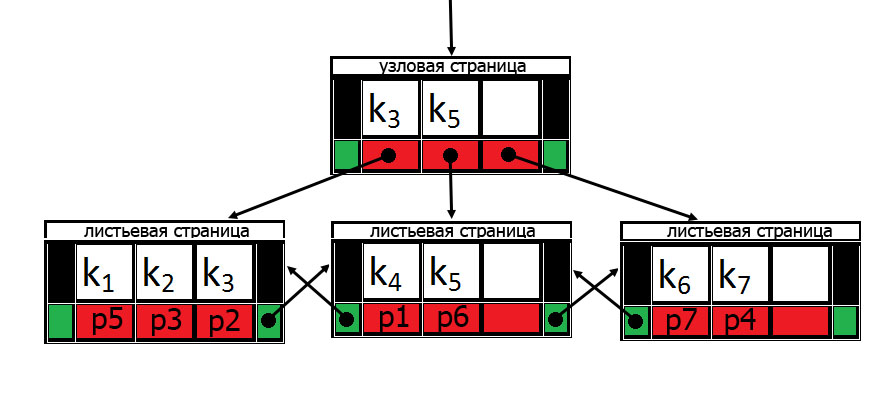
\includegraphics[scale=0.5]{index-structure.png}
  \caption{Структура вторичного индекса}
  \label{img:index-structure}
\end{figure}

\subsection{Составной индекс}

Чтобы правильно использовать составные индексы, необходимо понять структуру их хранения. Все работает точно так же, как и для обычного индекса, но для значений используются значения всех входящих колонок сразу, по которым строится индекс. Составной индекс может использоваться частично, но только по самому левому префиксу.

Если построить индекс по полям $(dob, last\_name)$, то для рисунка \ref{img:index-structure}
$k_1$ = 1799Пушкин, $k_2$ = 1814Лермонтов, $k_3$ = 1820Фет, $\ldots$

Составной индекс может использоваться как \textbf{частичный индекс}, являющийся левым префиксом составного индекса. 

\subsection{Селективность индексов}

Чем меньше строк войдет в выборку, тем быстрее будет работать поиск по ней. Если рассматривать таблицы с равномерно распределенными значениями в полях, то условие $=$ более селективно, чем условия $>$, $<=$, $>=$, $<$.

\subsection{Покрывающий индекс}
\label{section:covering-index}

Индекс называется покрывающим, если в нем есть все поля, используемые в запросе. Покрывающие индексы позволяют имитировать кластерные индексы. 

Для запроса на листинге \ref{sql:covering-index} строим индекс $(last\_name, dob)$.
\begin{lstlisting}[language=sql, label=sql:covering-index, caption={запрос для covering-index}]
SELECT last_name, dob
FROM poet
WHERE last_name = "Пушкин"
\end{lstlisting}
